% !Mode:: "TeX:UTF-8"

\titlecontents{chapter}[2em]{\vspace{.5\baselineskip}\xiaosan\song}%
             {\prechaptername\CJKnumber{\thecontentslabel}\postchaptername\qquad}{} %
             {}             % 设置该选项为空是为了不让目录中显示页码          
\addcontentsline{toc}{chapter}{外文资料}
%\setcounter{page}{1}       % 如果需要从该页开始从 1 开始编页,则取消该注释
\markboth{外文资料}{外文资料}
\chapter*{外文资料}

\includepdf[pages=-]{include/english.pdf}

% \begin{figure}[!b]
%     \centering
%     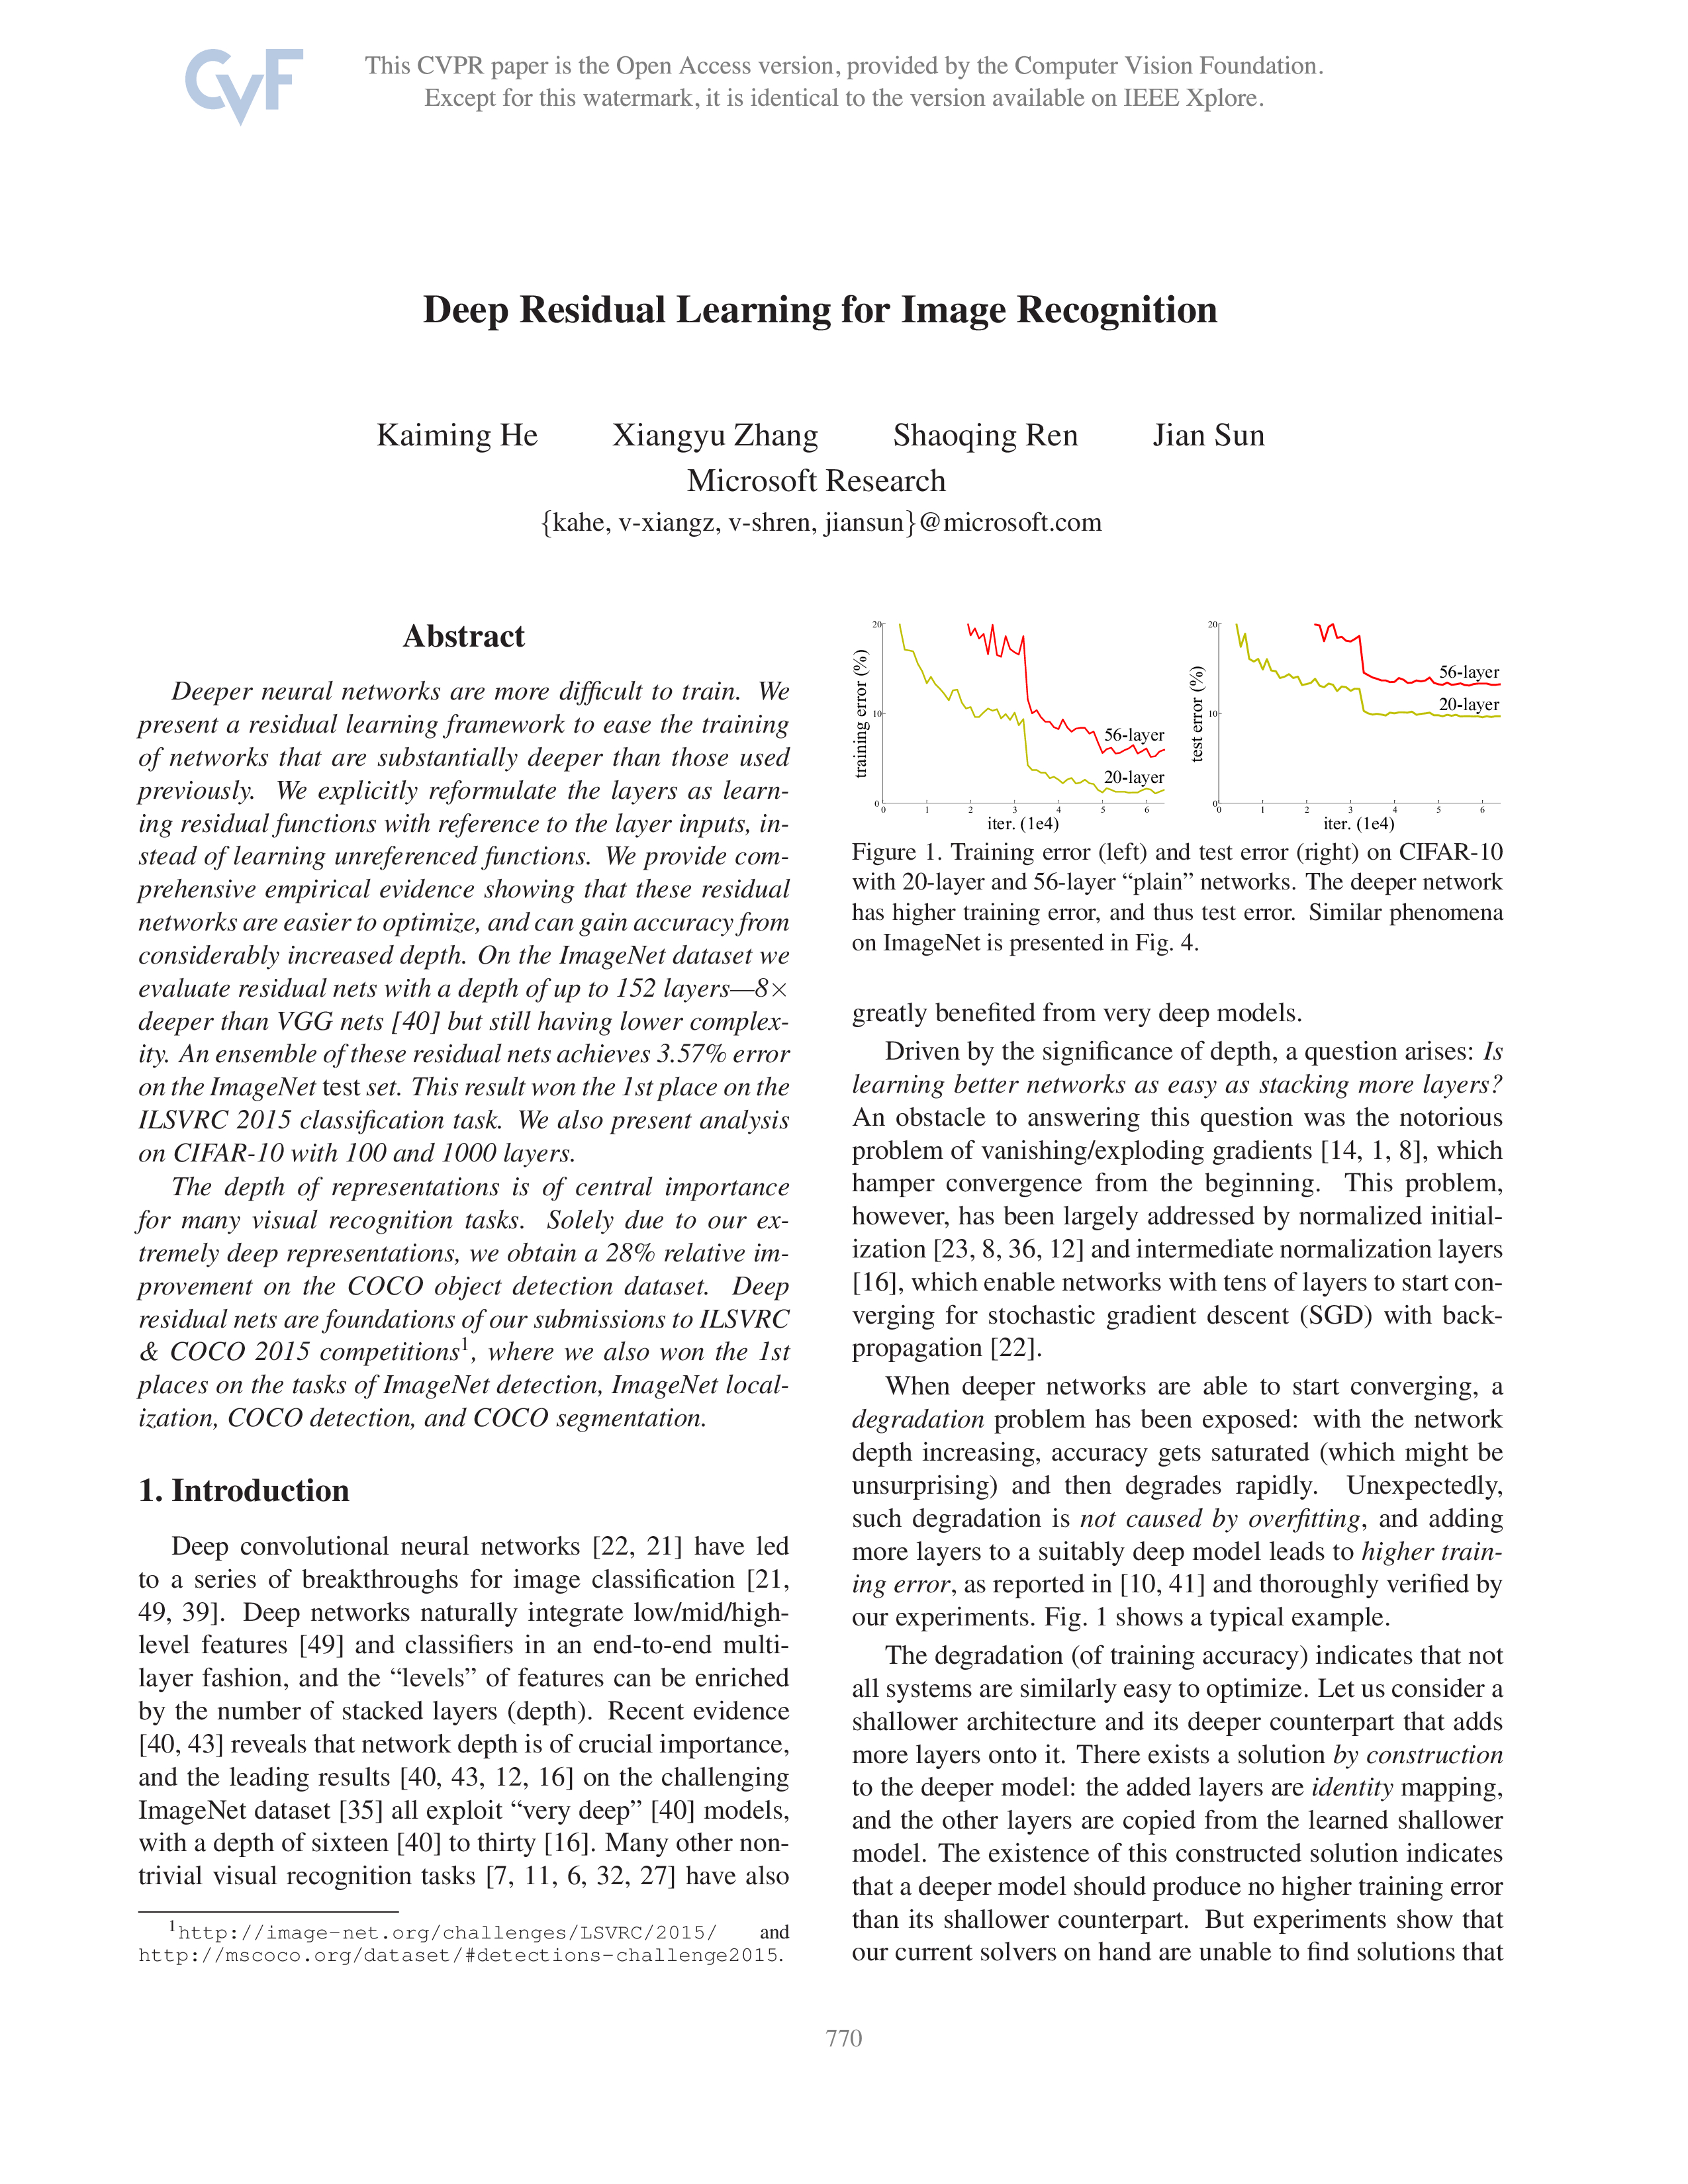
\includegraphics[width=\textwidth]{figures/english/english-0.jpg}
% \end{figure}

% \newpage

% \begin{figure}[!tbp]
%     \centering
%     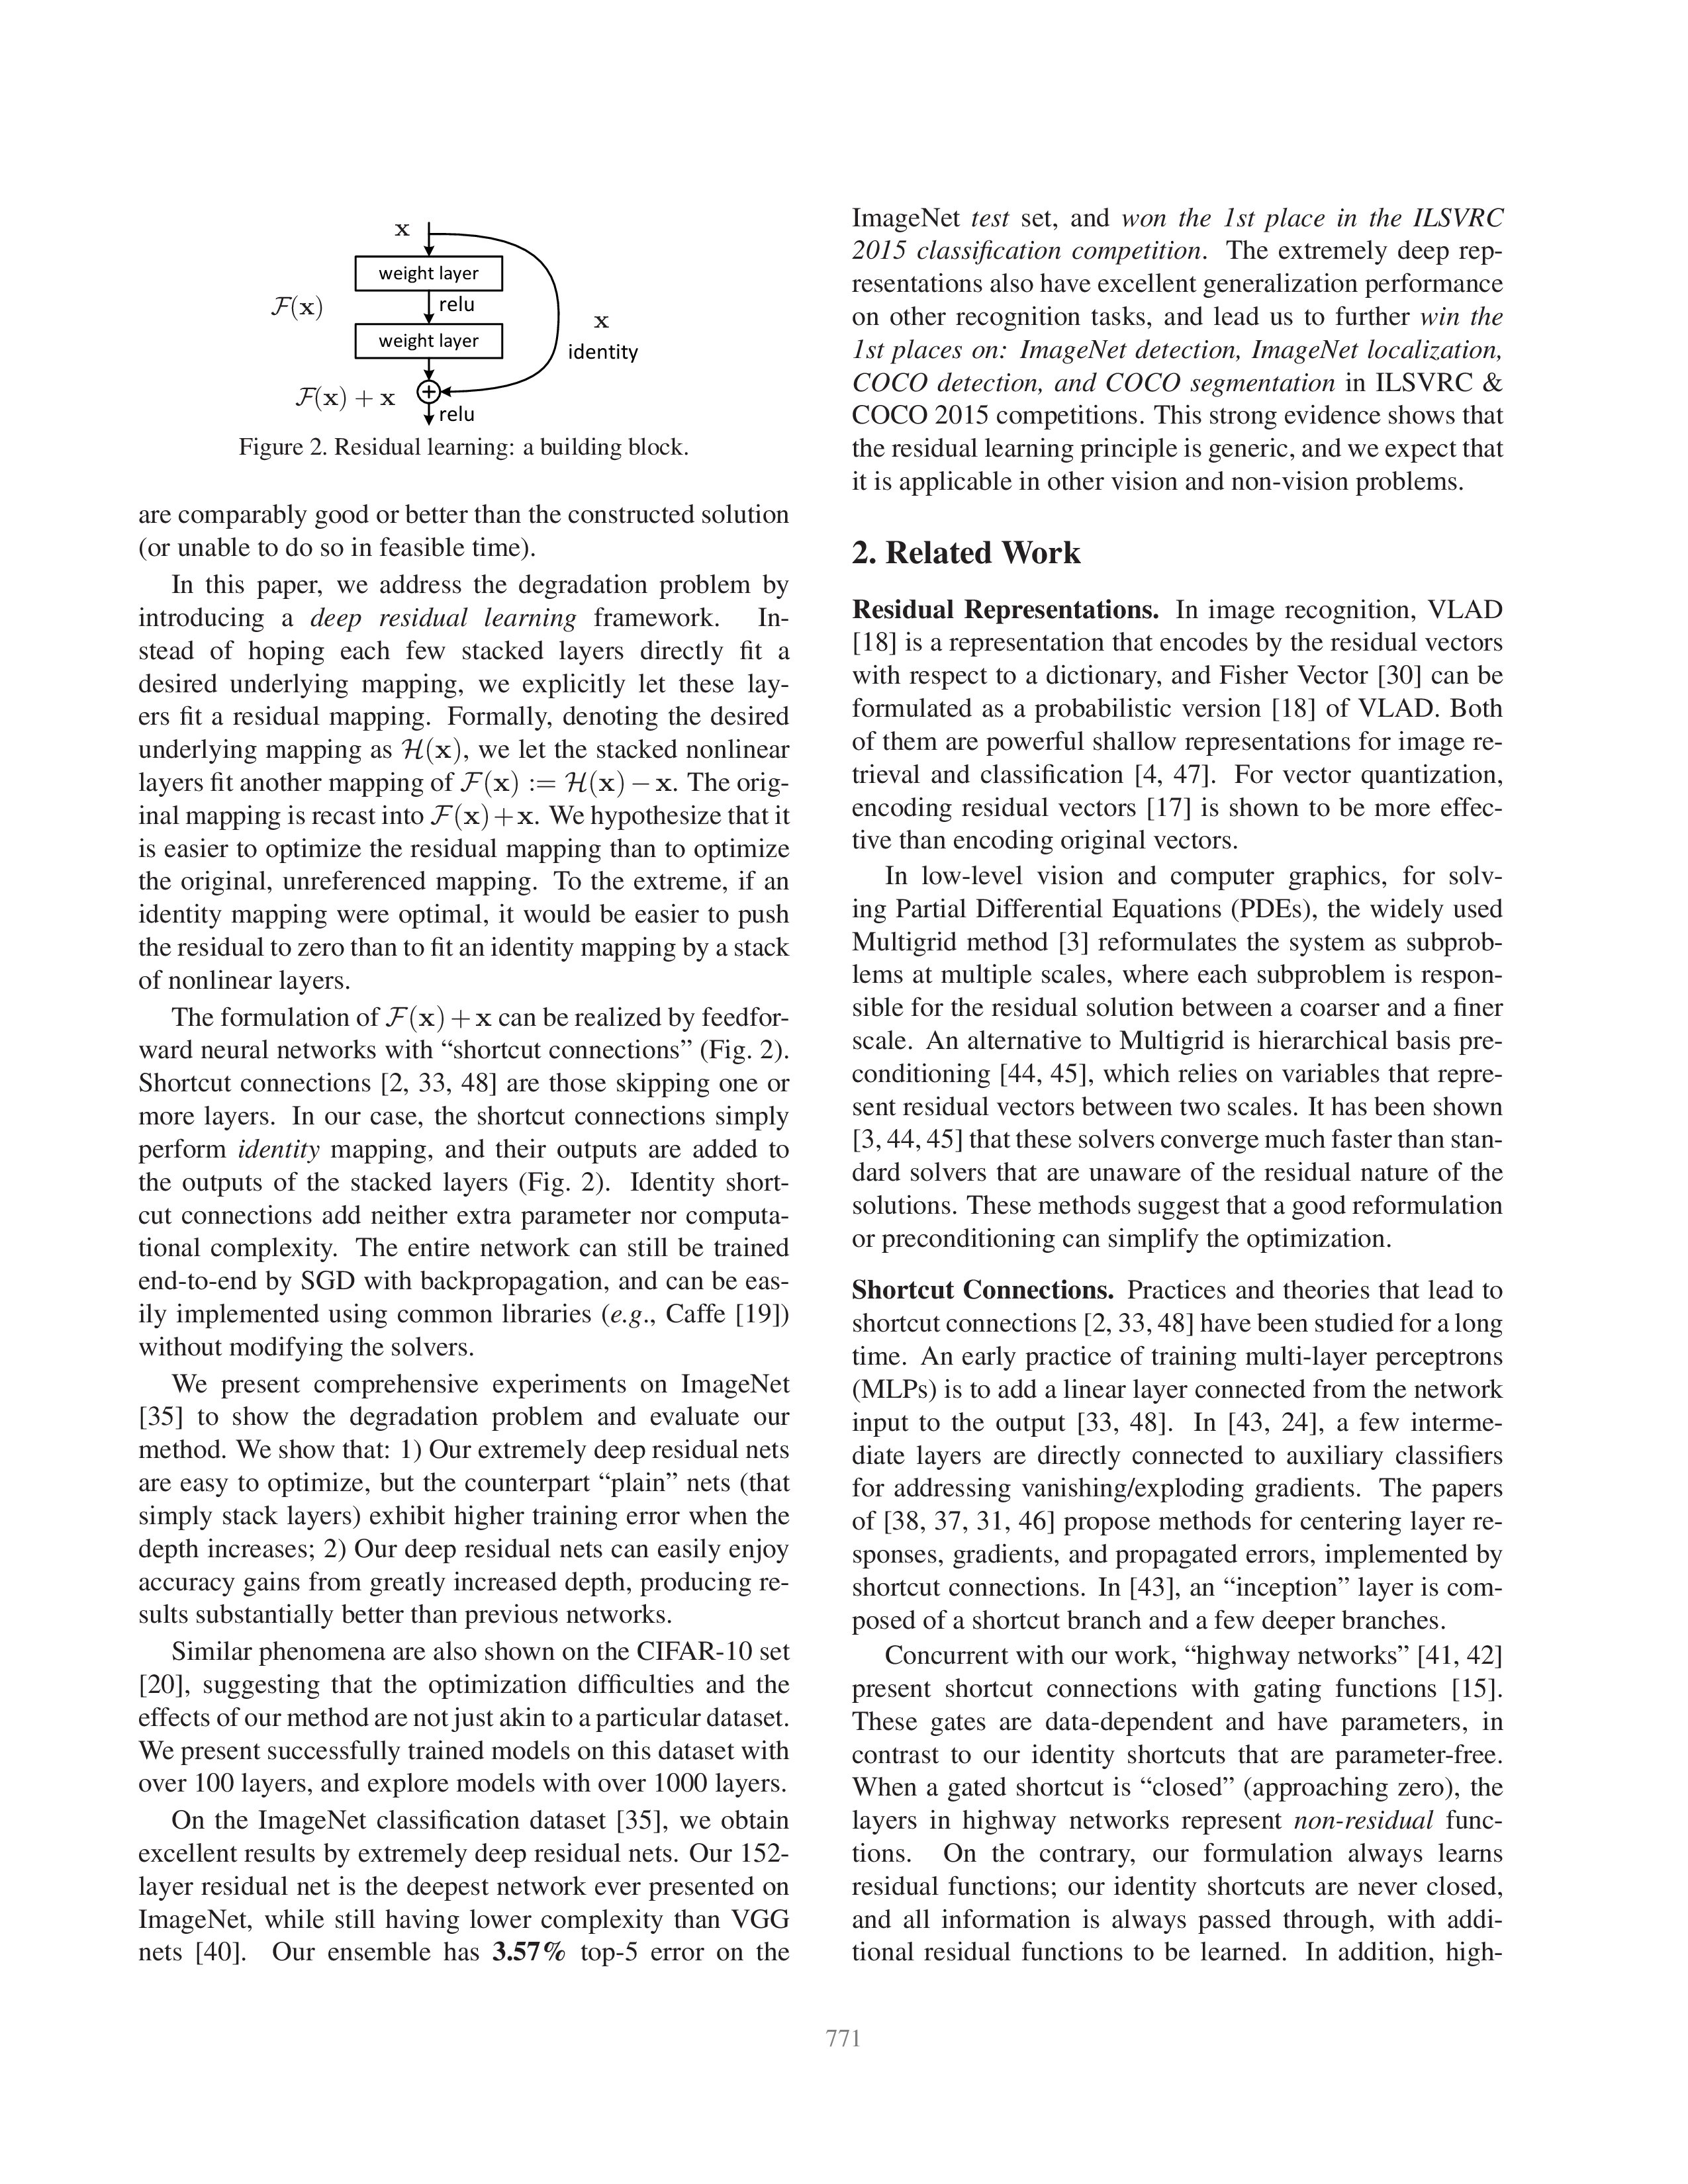
\includegraphics[width=\textwidth]{figures/english/english-1.jpg}
% \end{figure}

% \begin{figure}[!tbp]
%     \centering
%     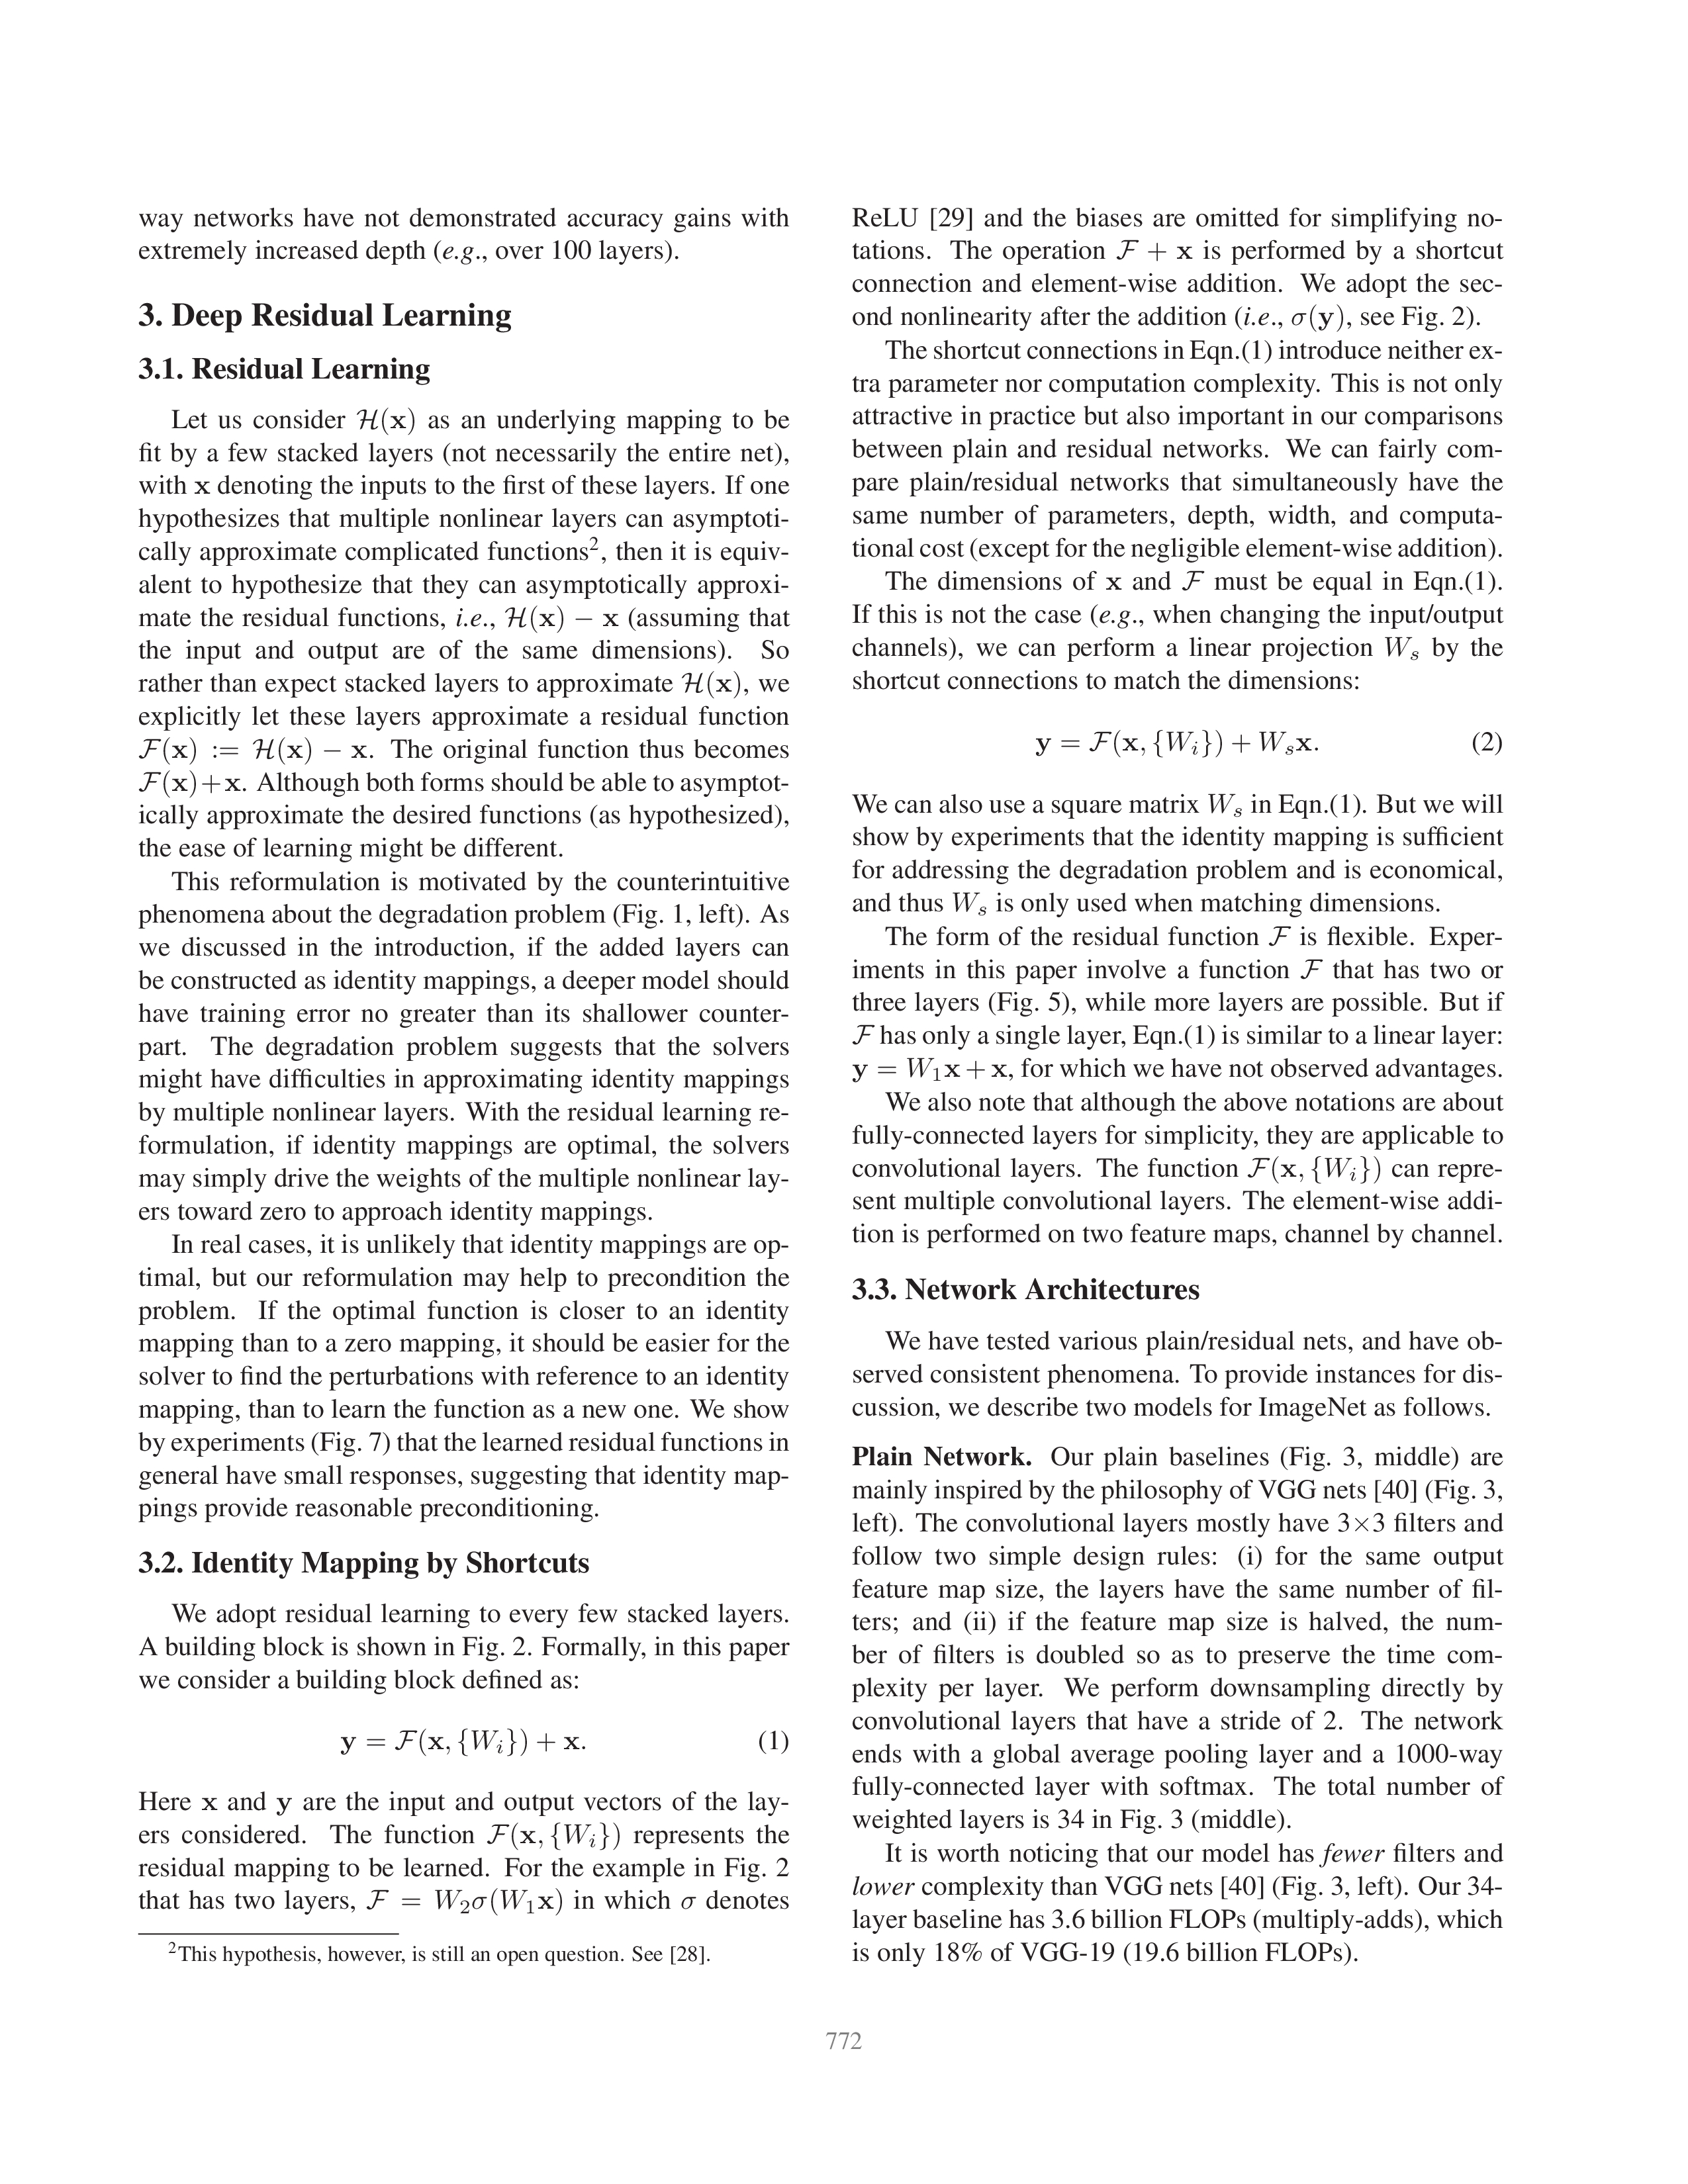
\includegraphics[width=\textwidth]{figures/english/english-2.jpg}
% \end{figure}

% \begin{figure}[!tbp]
%     \centering
%     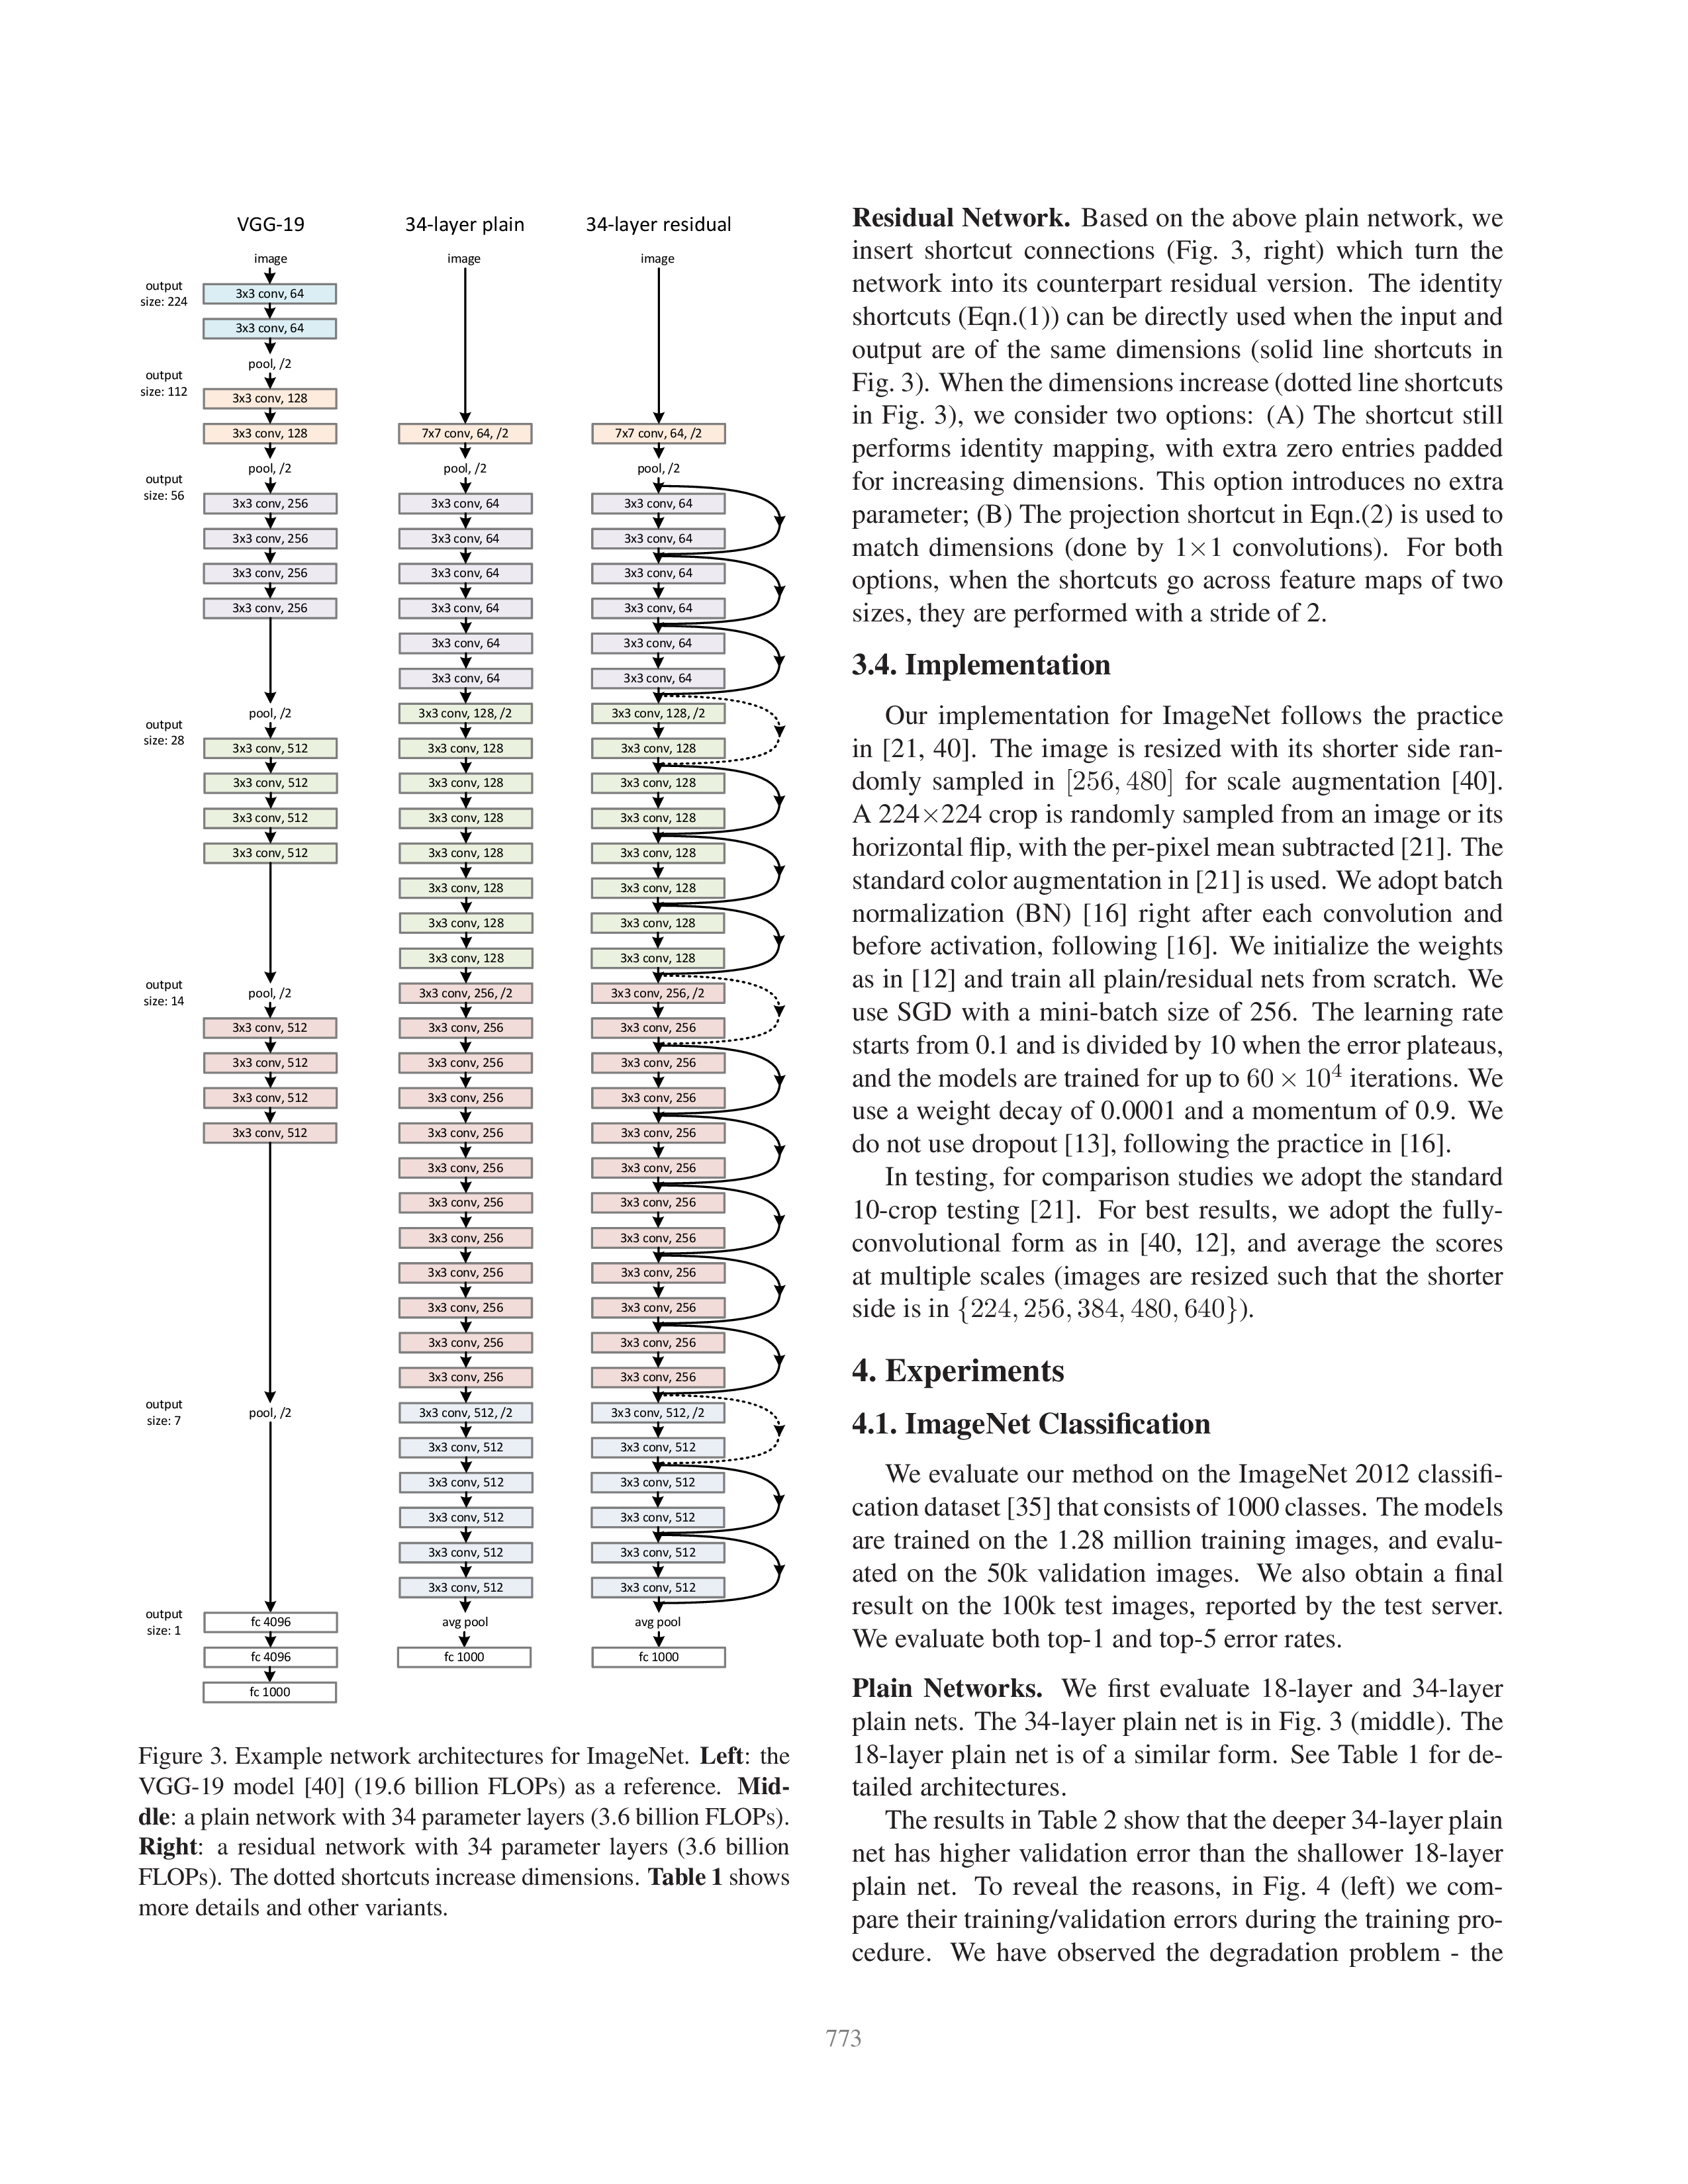
\includegraphics[width=\textwidth]{figures/english/english-3.jpg}
% \end{figure}

% \begin{figure}[!tbp]
%     \centering
%     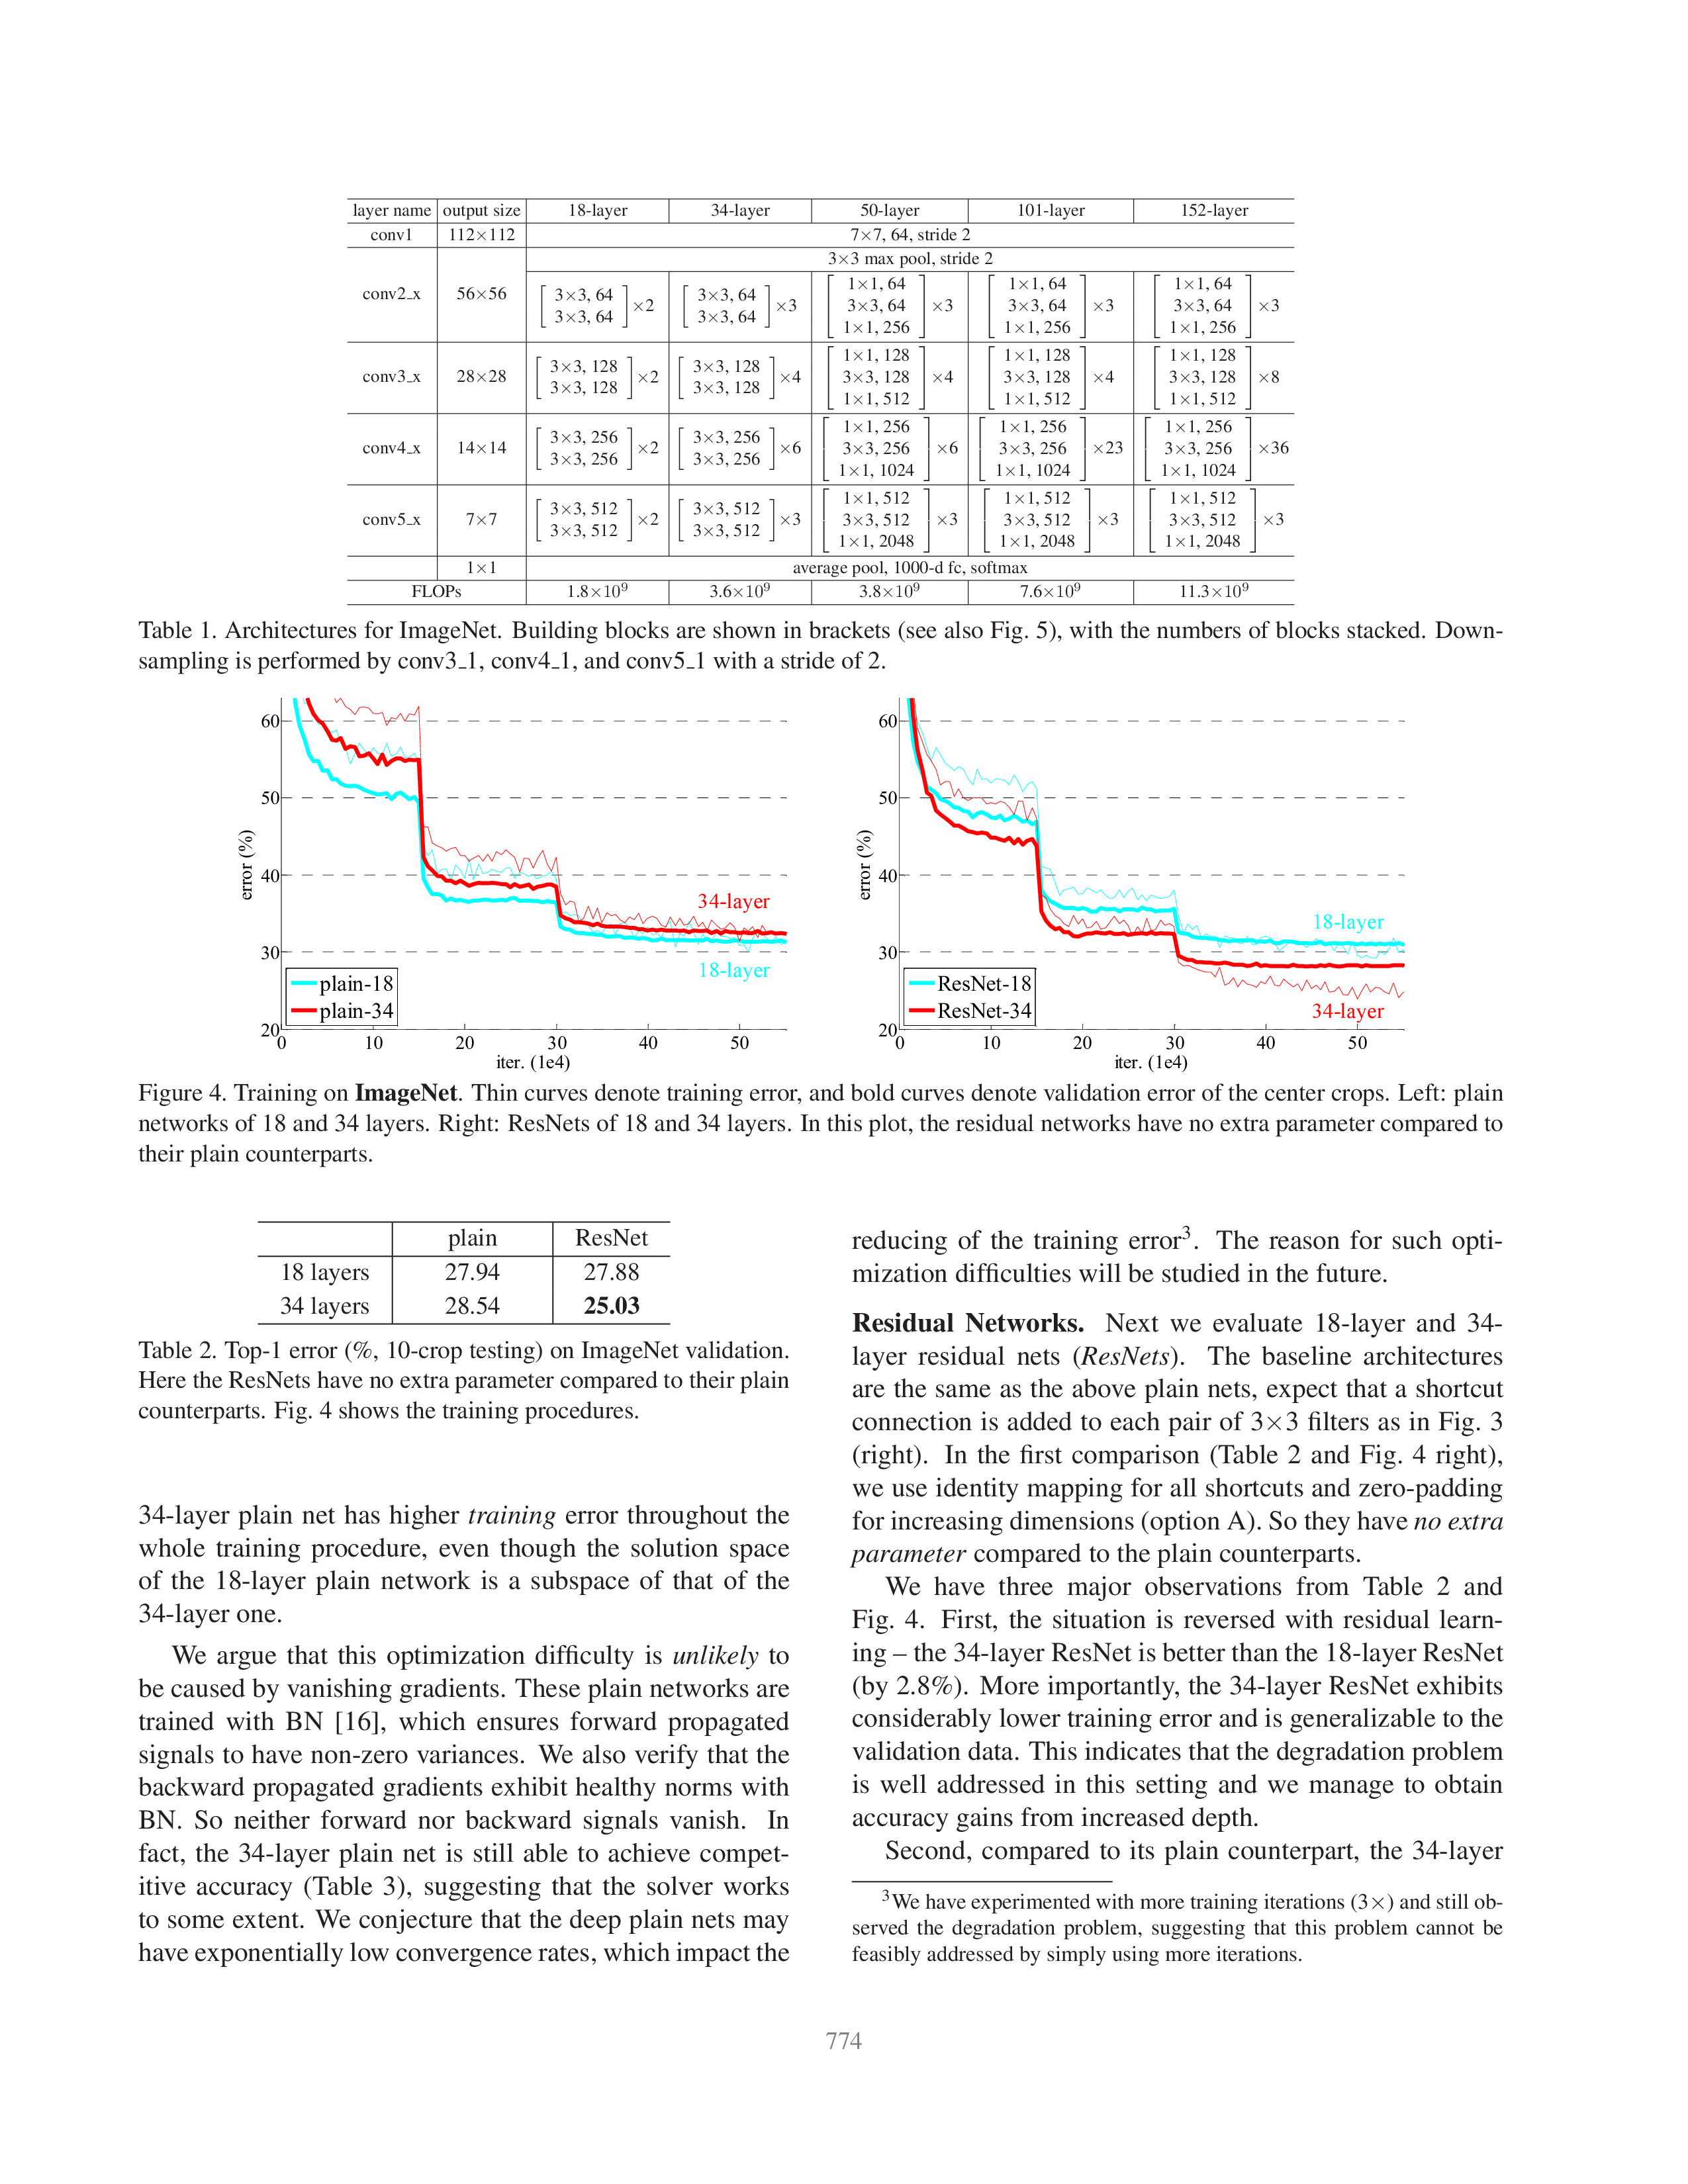
\includegraphics[width=\textwidth]{figures/english/english-4.jpg}
% \end{figure}

% \begin{figure}[!tbp]
%     \centering
%     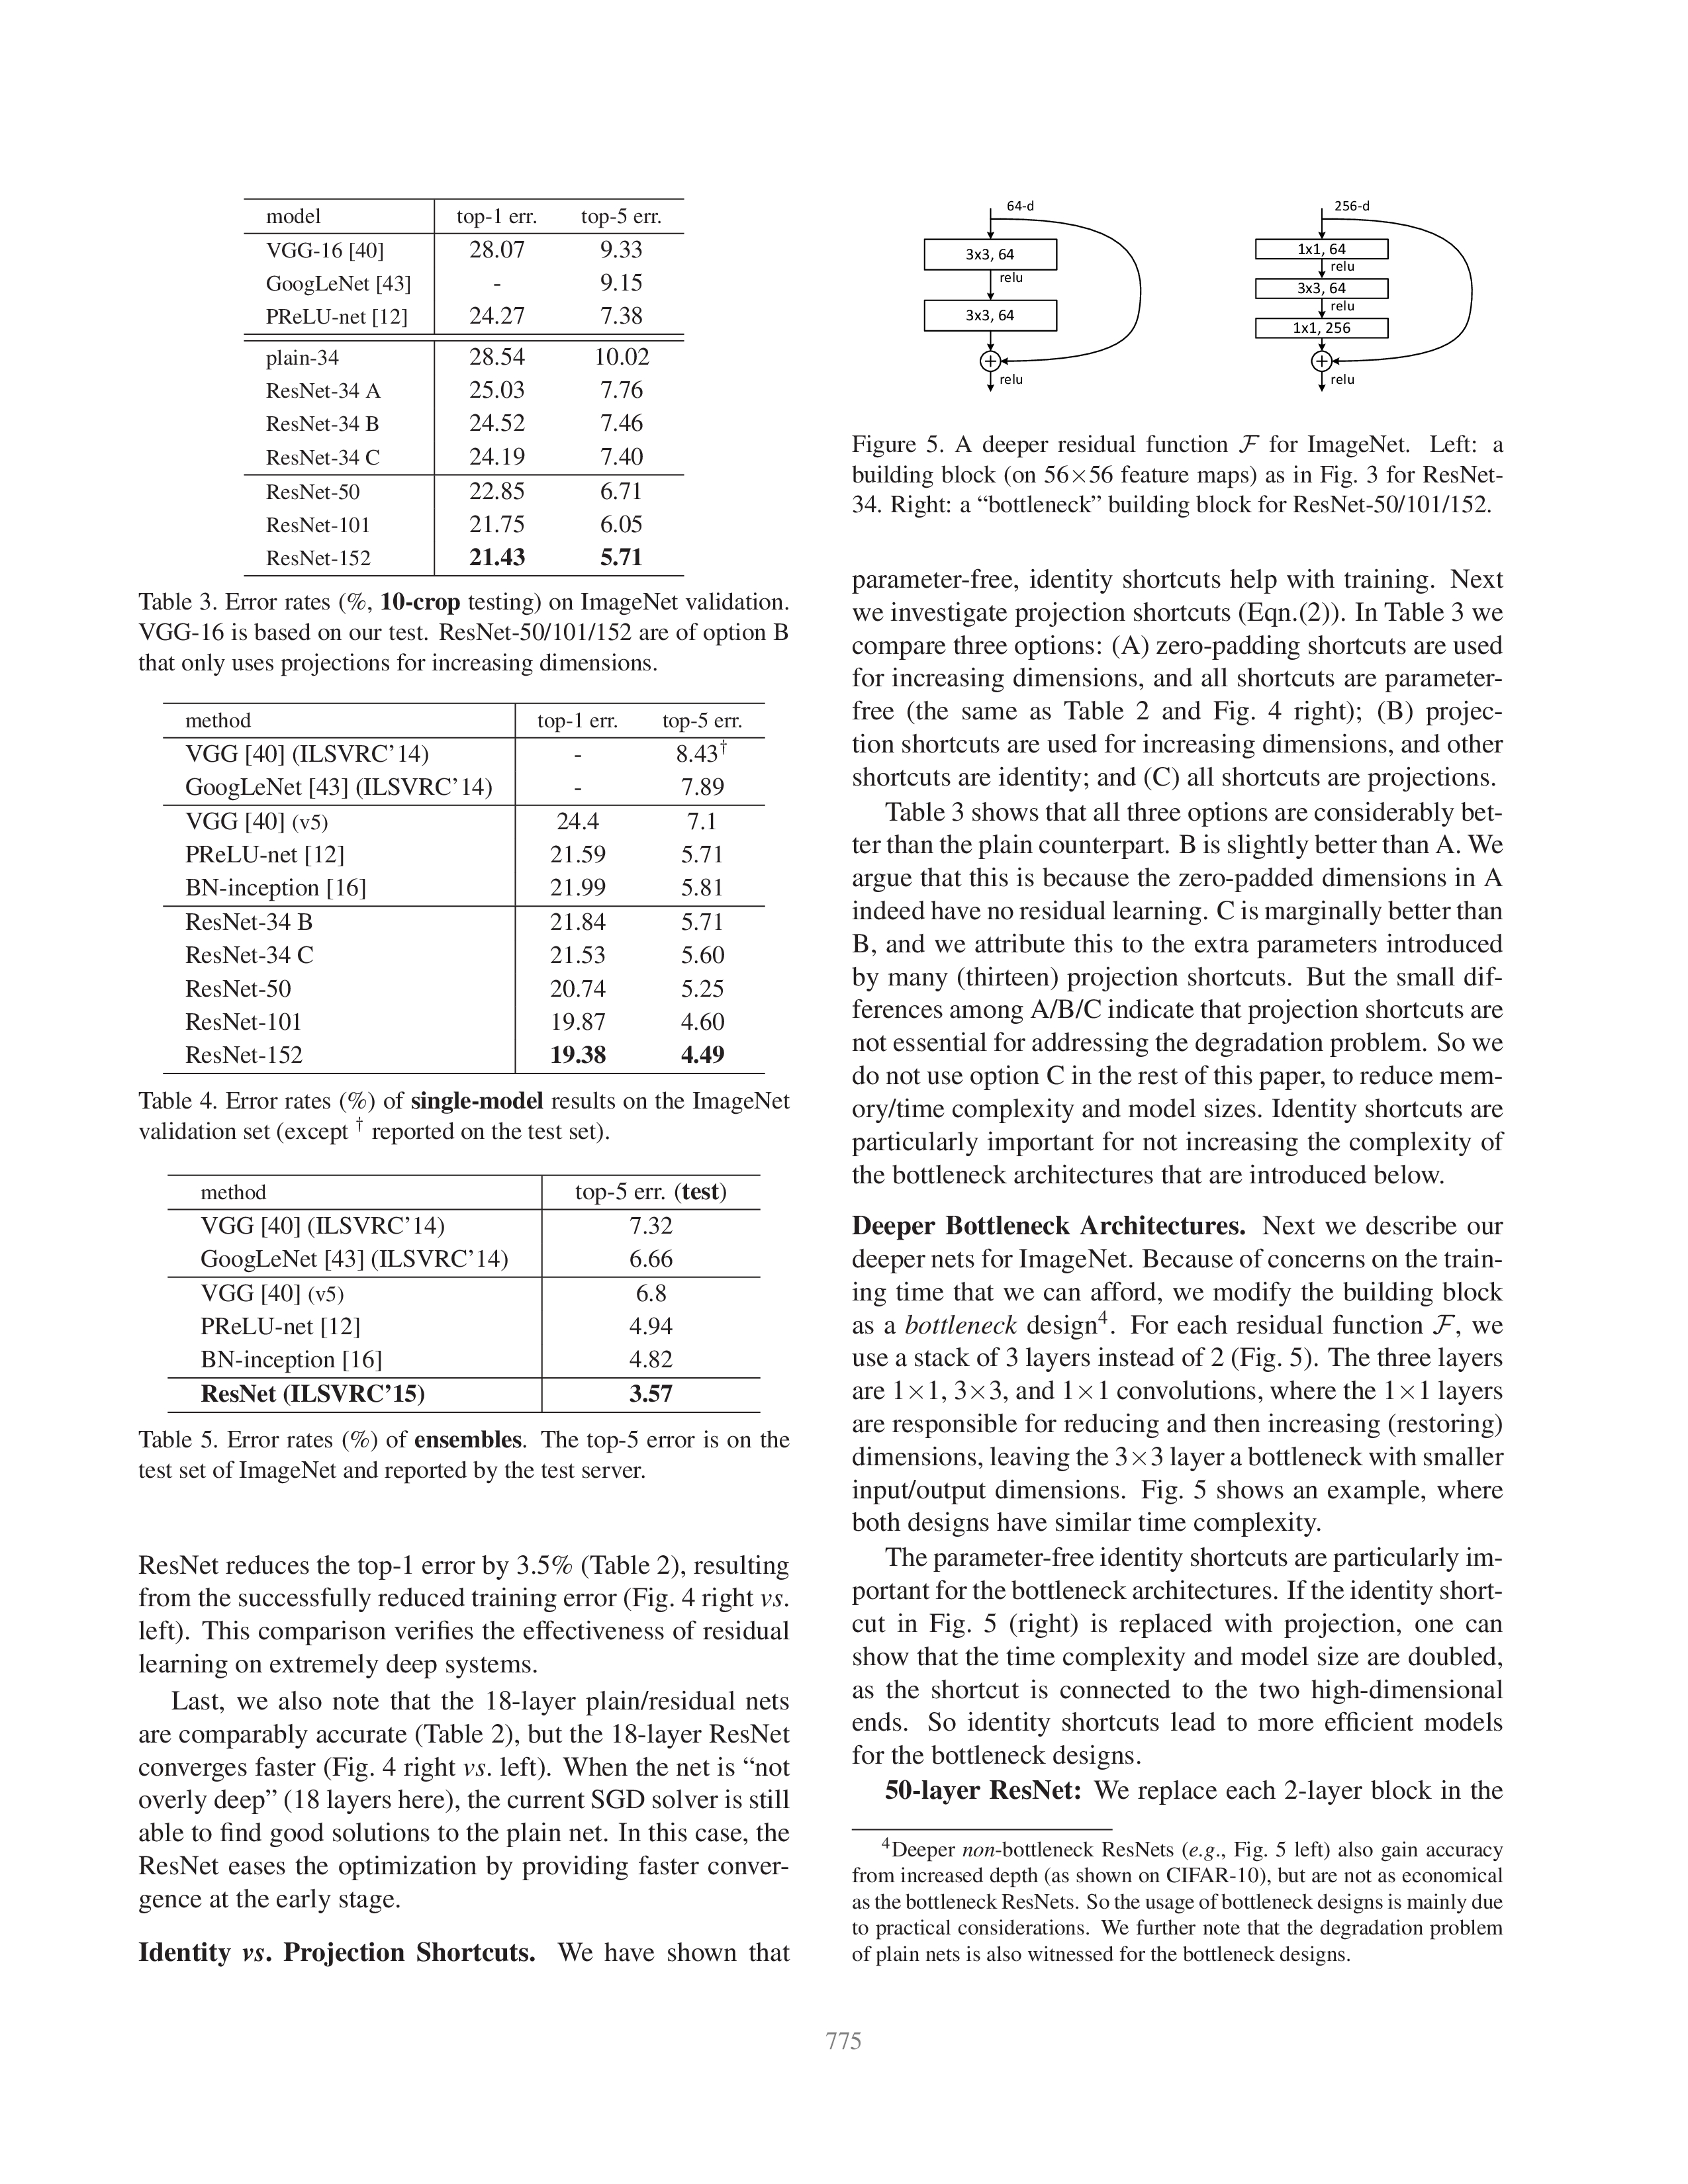
\includegraphics[width=\textwidth]{figures/english/english-5.jpg}
% \end{figure}

% \begin{figure}[!tbp]
%     \centering
%     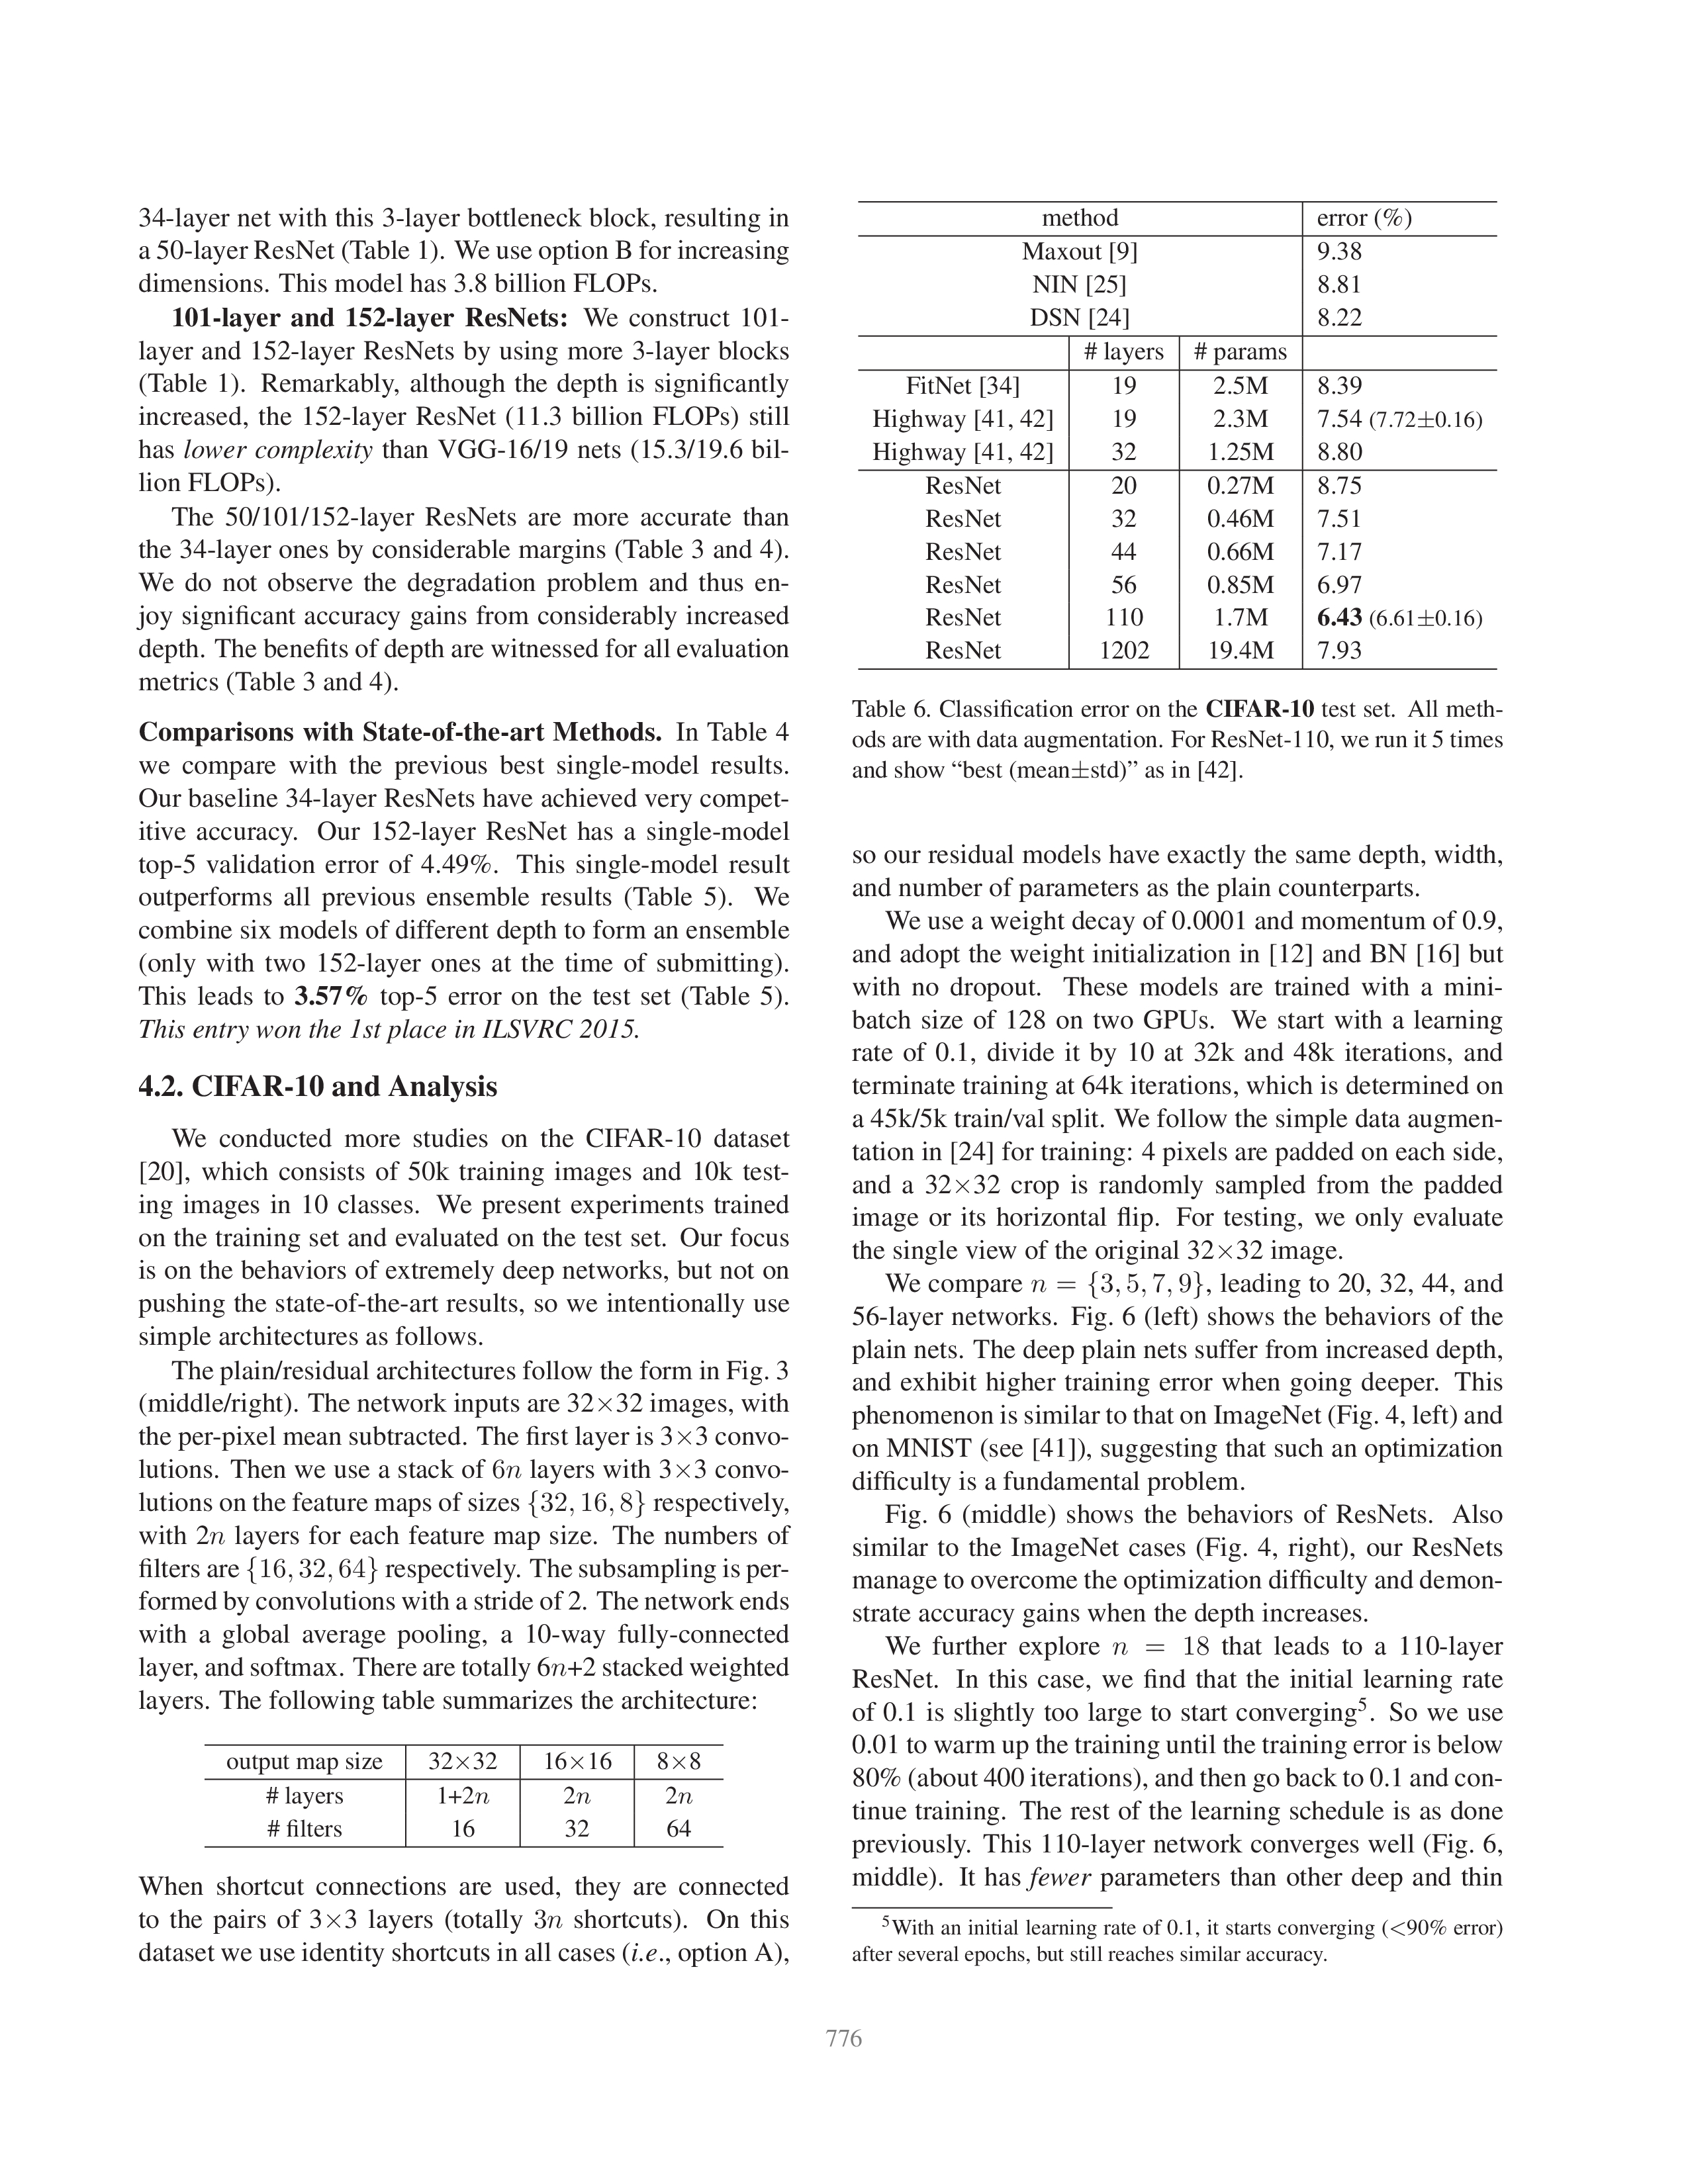
\includegraphics[width=\textwidth]{figures/english/english-6.jpg}
% \end{figure}

% \begin{figure}[!tbp]
%     \centering
%     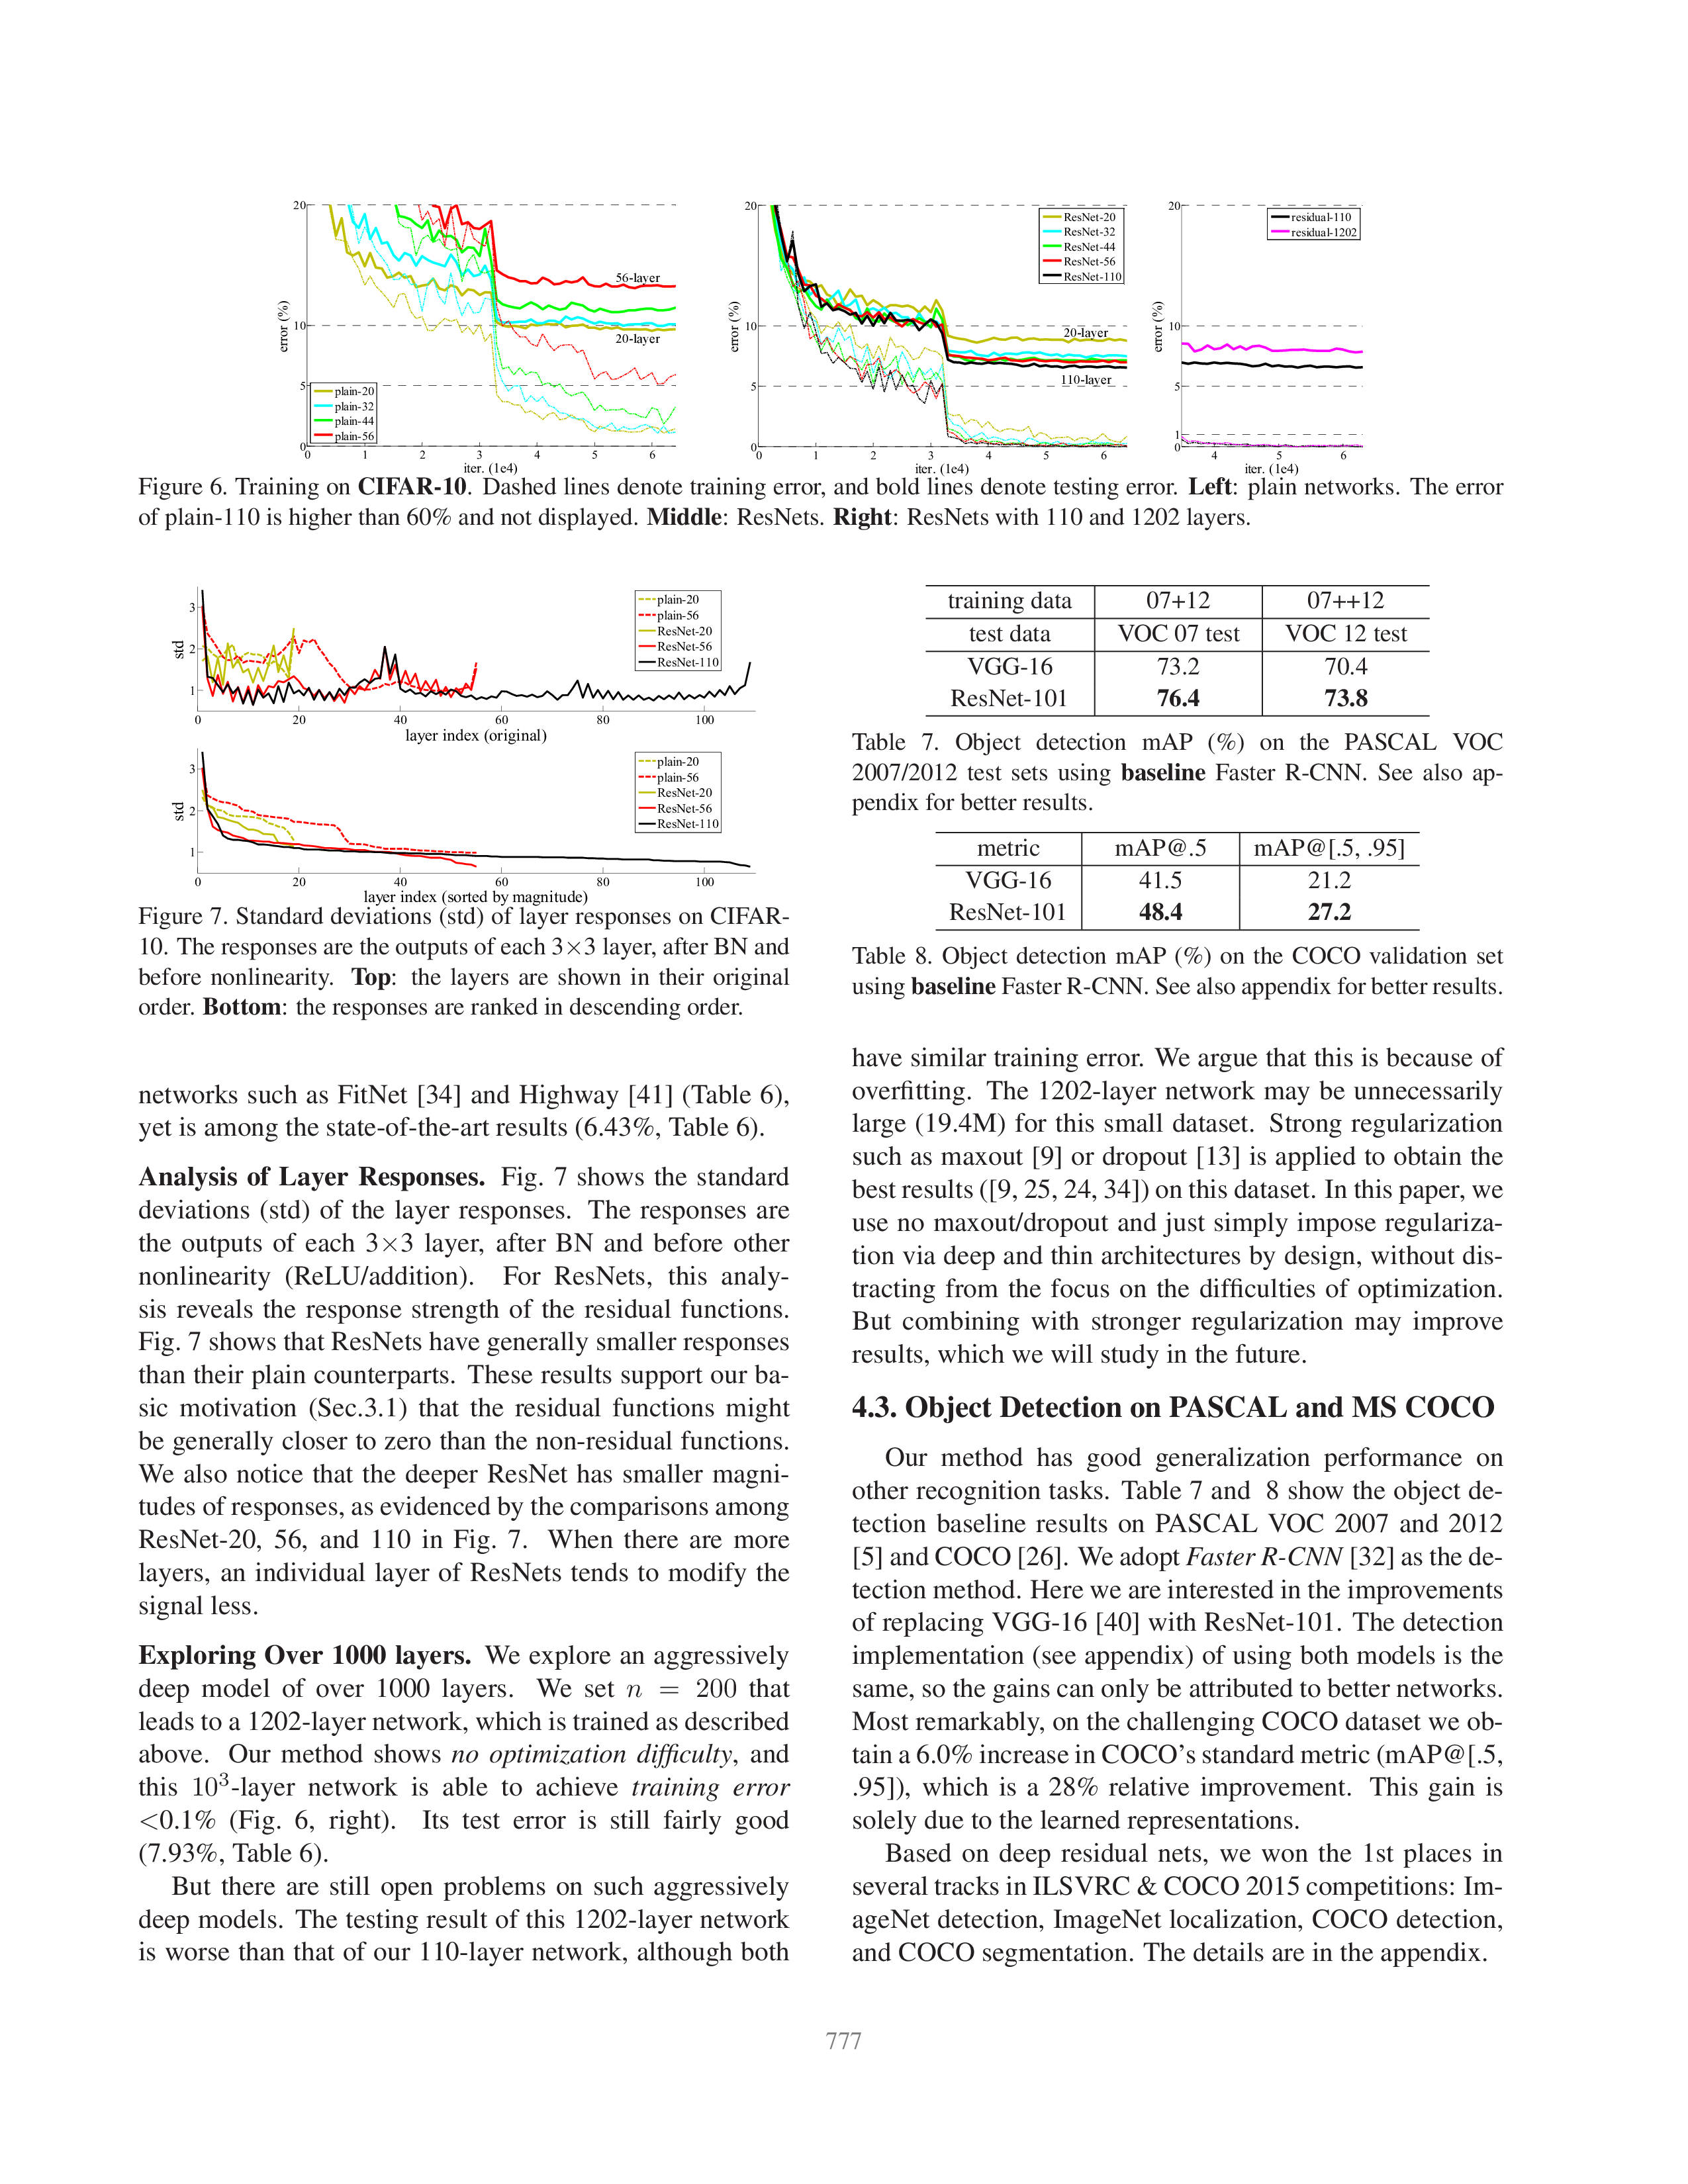
\includegraphics[width=\textwidth]{figures/english/english-7.jpg}
% \end{figure}

% \begin{figure}[!tbp]
%     \centering
%     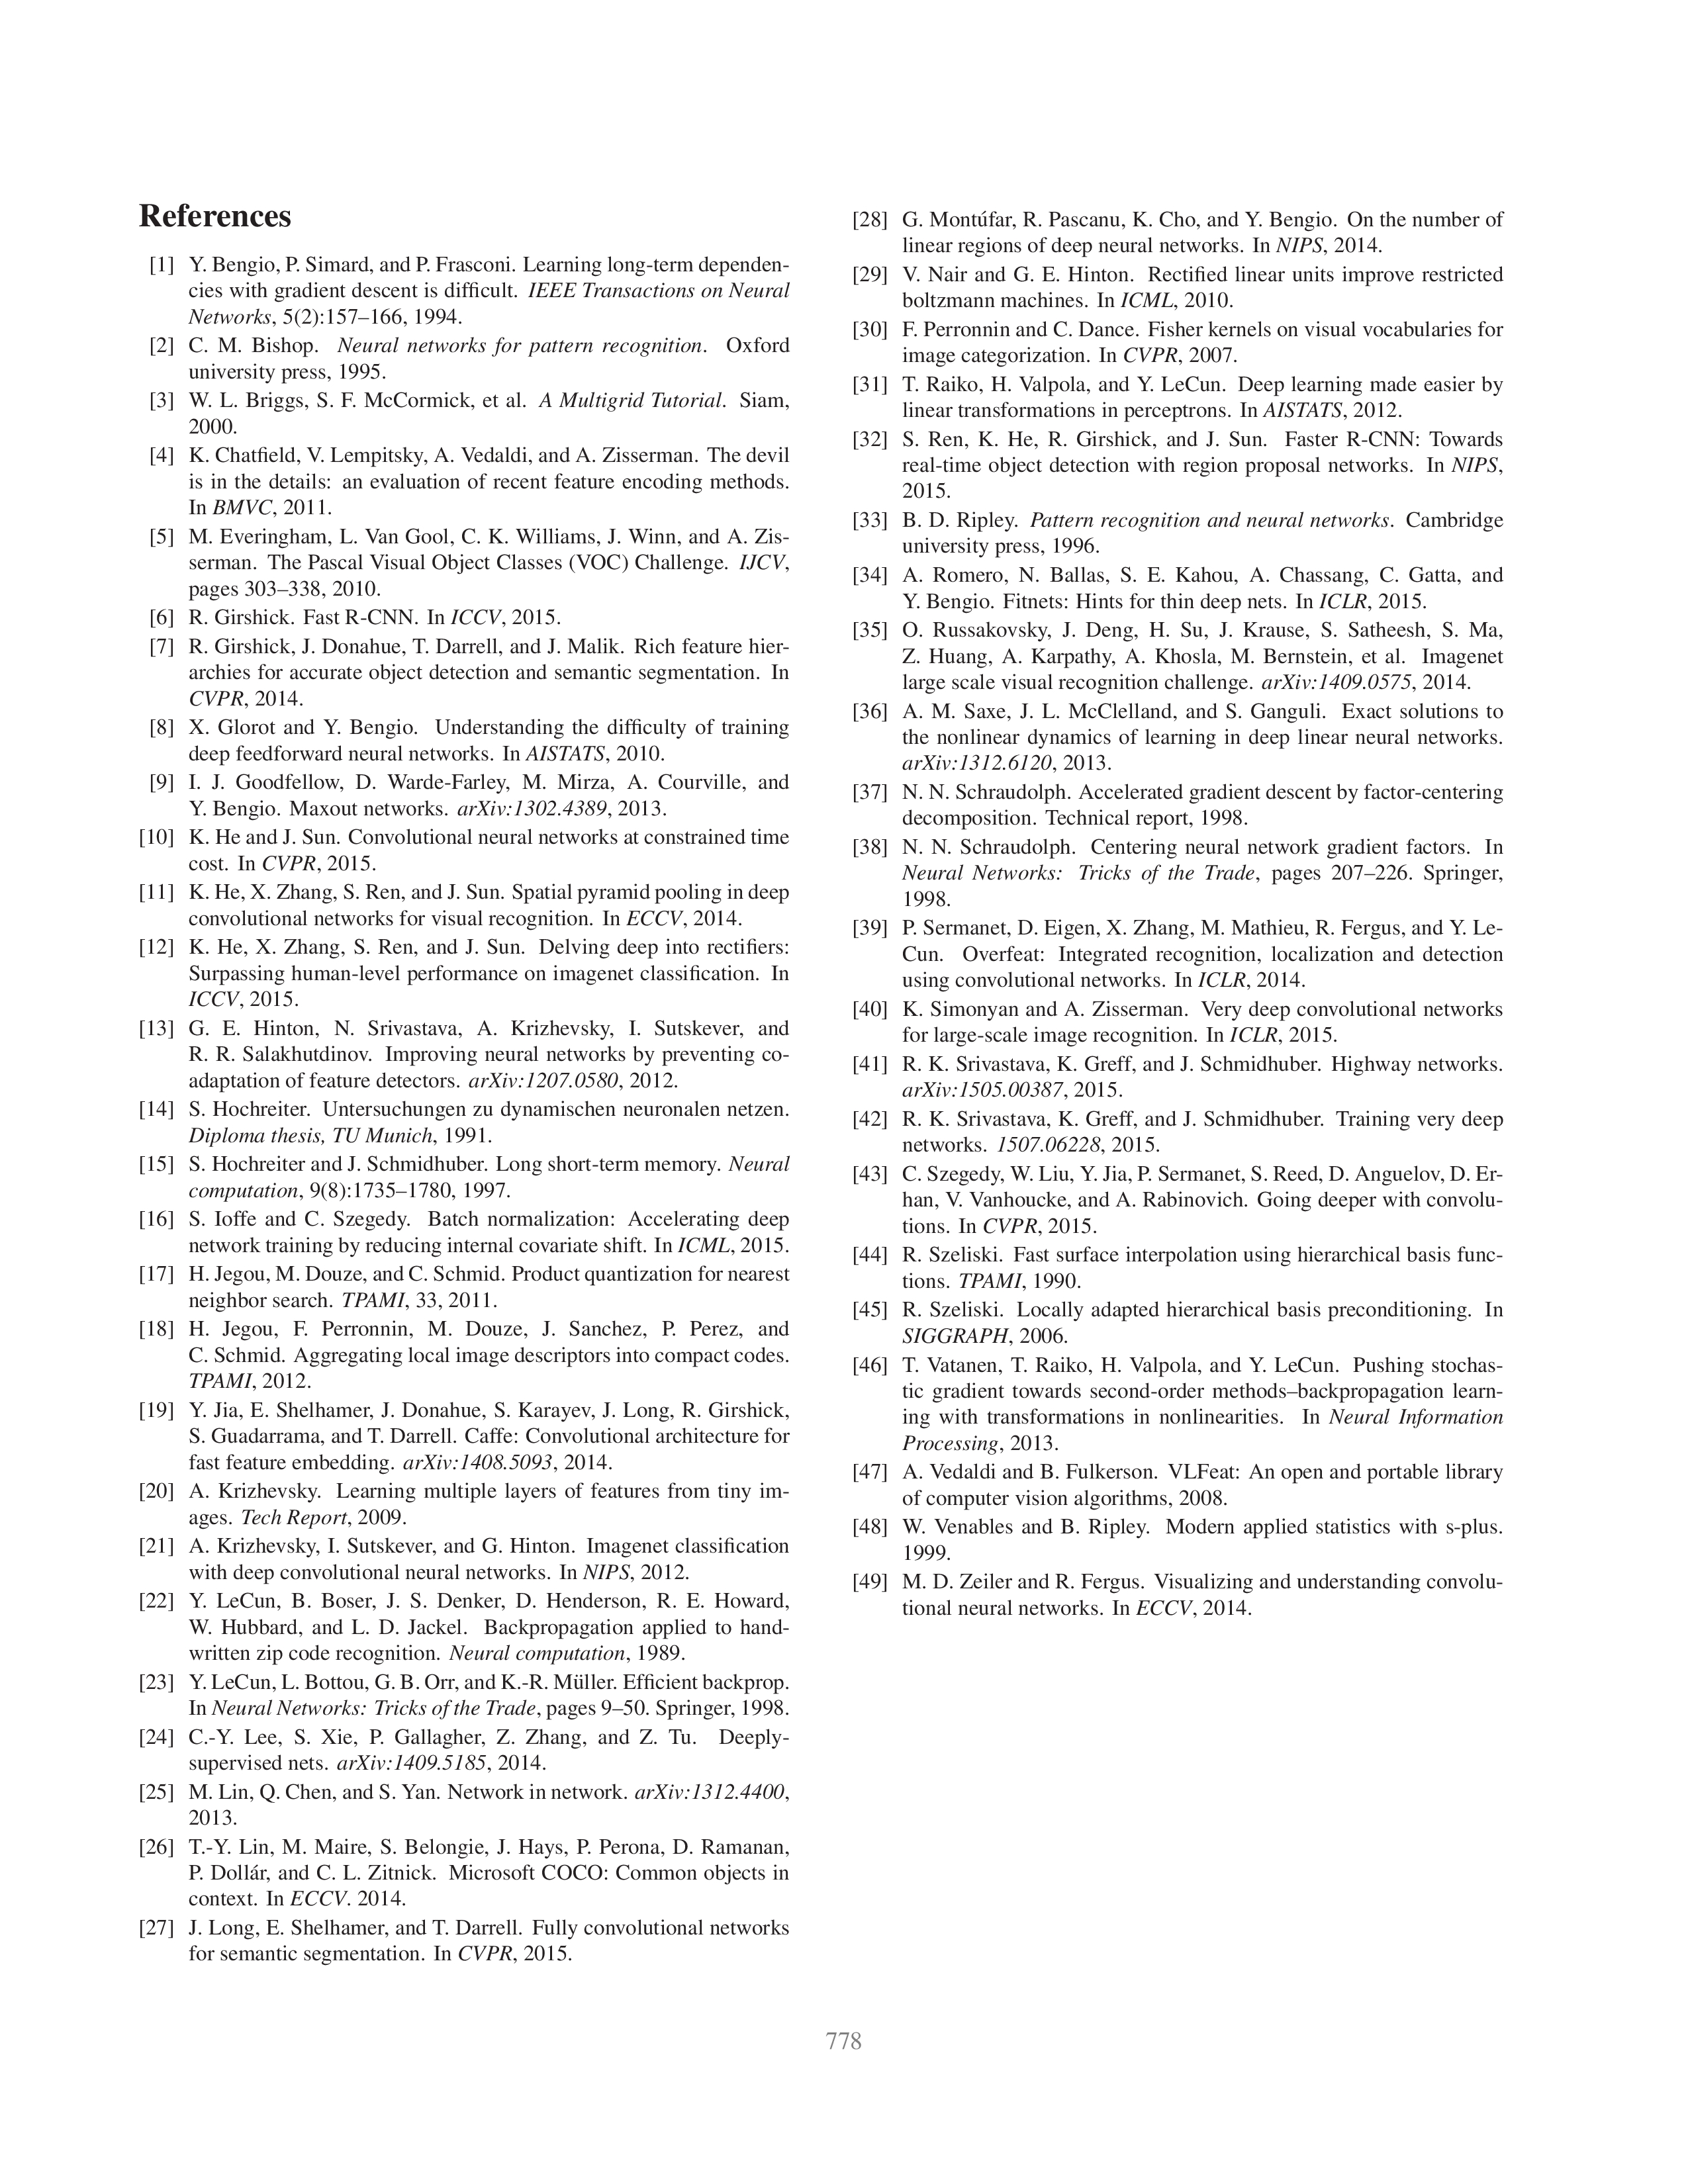
\includegraphics[width=\textwidth]{figures/english/english-8.jpg}
% \end{figure}